\documentclass[lettersize,journal]{IEEEtran}
\usepackage{amsmath,amsfonts}
\usepackage{algorithmic}
\usepackage{algorithm}
\usepackage{array}
\usepackage[caption=false,font=normalsize,labelfont=sf,textfont=sf]{subfig}
\usepackage{textcomp}
\usepackage{stfloats}
\usepackage{url}
\usepackage{verbatim}
\usepackage{graphicx}
\usepackage{cite}

% added packages from authors
\usepackage{xcolor}
\usepackage{booktabs} % for \midrule in tables
\usepackage{hhline}
\usepackage{bbm}
\usepackage{bm}
\usepackage{makecell}
\usepackage[mode=buildnew]{standalone}
\usepackage{tikz}
\usetikzlibrary{calc,arrows,patterns,intersections}
\usepackage{pgfplots}
\usepackage{xcolor}
\usepgfplotslibrary{fillbetween}

\hyphenation{op-tical net-works semi-conduc-tor IEEE-Xplore}

\begin{document}


\title{A New Paradigm for Energy Intensive Industries: Adapting to Provide Power Flexibility}

\author{Peter A.V. Gade\textsuperscript{*}\textsuperscript{\textdagger}, Trygve Skjøtskift\textsuperscript{\textdagger}, Charalampos Ziras\textsuperscript{*}, Henrik W. Bindner\textsuperscript{*}, Jalal Kazempour\textsuperscript{*} \\
    \textsuperscript{*}Department of Wind and Energy Systems, Technical University of Denmark, Kgs. Lyngby, Denmark \\
    \textsuperscript{\textdagger}IBM Client Innovation Center, Copenhagen, Denmark
    % <-this % stops a space
    \thanks{Corresponding author. Tel.: +45 24263865. \\ Email addresses: pega@dtu.dk (P.A.V. Gade), Trygve.Skjotskift@ibm.com (T. Skjøtskift), hwbi@dtu.dk (H.W. Bindner), jalal@dtu.dk (J. Kazempour).}% <-this % stops a space
    \thanks{Manuscript received April 19, 2021; revised August 16, 2021.}}

% \footnote{Corresponding author. Tel.: +45 24263865. \\ Email addresses: pega@dtu.dk (P.A.V. Gade), Trygve.Skjotskift@ibm.com (T. Skjøtskift), hwbi@dtu.dk (H.W. Bindner), jalal@dtu.dk (J. Kazempour).}

% The paper headers
\markboth{Journal of \LaTeX\ Class Files,~Vol.~14, No.~8, August~2021}%
{Shell \MakeLowercase{\textit{et al.}}: A Sample Article Using IEEEtran.cls for IEEE Journals}

\IEEEpubid{0000--0000/00\$00.00~\copyright~2021 IEEE}
% Remember, if you use this you must call \IEEEpubidadjcol in the second
% column for its text to clear the IEEEpubid mark.

\maketitle

% \tableofcontents

\begin{abstract}
    \input{sections/abstract}
\end{abstract}

\begin{IEEEkeywords}
    Demand-side flexibility.
\end{IEEEkeywords}

\section{Introduction}
% \IEEEpubidadjcol


\subsection{Research questions}

\begin{itemize}
    \item Is there incentives for an energy intensive industry process position deliver power  flexibility to the grid?
    \item How can it adapt to provide power flexibility?
    \item What types of flexibility are well suited to an energy intensive industry process?
\end{itemize}

\subsection{Investments should facilitate power flexibility}

\subsection{Value streams from power flexibility: FCR and mFRR}

\subsection{Literature review}

\subsection{Our contribution}

For an energy intensive industry process using real data from 2022, is there any incentive to provide power flexibility or to invest in equipment for the enablement of flexibility provision? We investigate those questions with a specific focus on mFRR and FCR in DK1 in Denmark. We provide an upper bound of flexibility earnings using a full hindsight optimization of each market. Each flexibility service is analyzed in terms of its impact on the process, in this case its impact on the temperature.

\section{Adapting an industry process to work as a TCL}

\subsubsection{Characterising a zinc furnace as a TCL}

\begin{figure}[!t]
    \centering
    \includestandalone[width=0.5\columnwidth]{figures/furnace_schematic_tikz}
    \caption{Schematic of the zinc furnace.}
    \label{fig:furnace_schematic_tikz}
\end{figure}

\begin{figure}[!t]
    \centering
    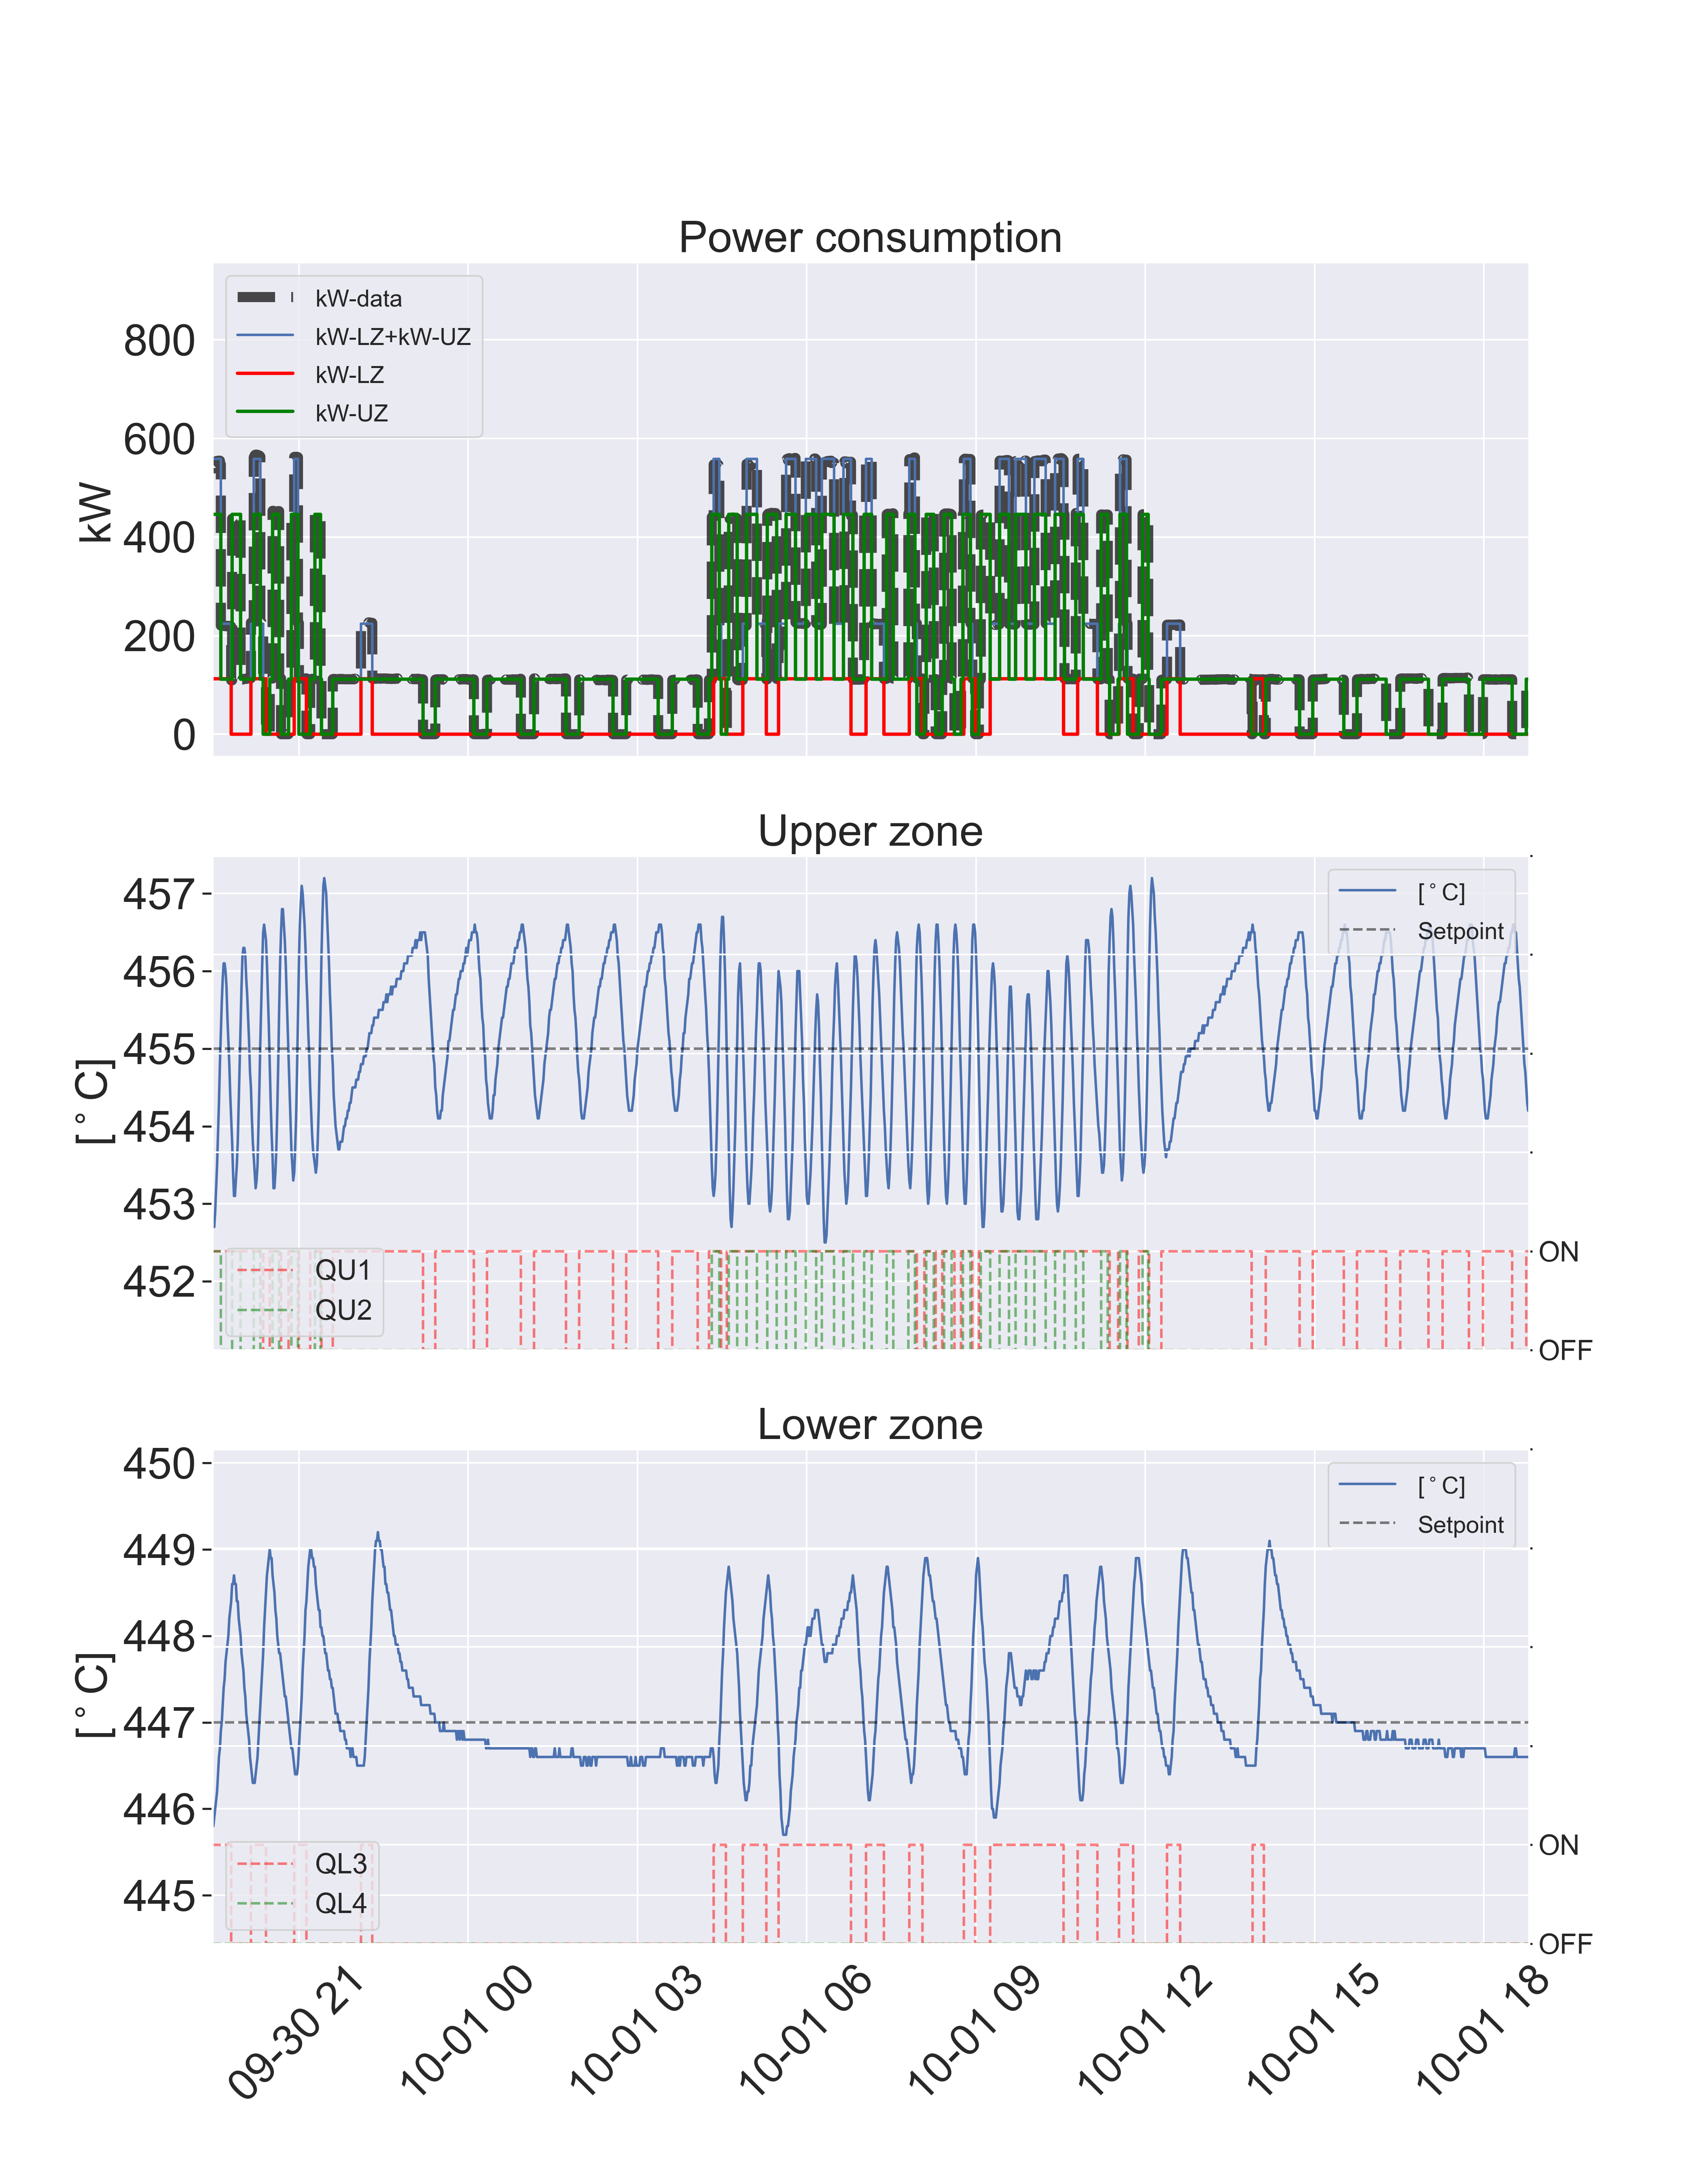
\includegraphics[width=\columnwidth]{figures/data_visualization.png}
    \caption{\textbf{Top}: Power consumption for lower and upper zone as well as total consumption. \textbf{Middle}: Temperature and contactor switches in upper zone. \textbf{Bottom}: Temperature and contactor switches in lower zone.}
    \label{fig:data_visualization}
\end{figure}

\begin{subequations}\label{eq:StateSpaceModel}
    \begin{align}
        T^{zu}_{t+1} & = T^{zu}_{t} + dt \cdot \frac{1}{C^{zu}}\Bigl( \frac{1}{R^{zuzl}} (T^{zl}_{t} - T^{zu}_{t}) \notag                            \\ & \mspace{5mu} + \frac{1}{R^{wz}} (T^{wu}_{t} - T^{zu}_{t}) \Bigr) \\
        T^{zl}_{t+1} & = T^{zl}_{t} + dt \cdot \frac{1}{C^{zl}}\Bigl( \frac{1}{R^{zuzl}} (T^{zu}_{t} - T^{zl}_{t}) \notag                            \\ & \mspace{5mu} + \frac{1}{R^{wz}} (T^{wl}_{t} - T^{zl}_{t}) \Bigr) \\
        T^{wu}_{t+1} & = T^{wu}_{t} + dt \cdot \frac{1}{C^{wu}}\Bigl( (1-\mathbbm{1}^{\text{lid}}) \frac{1}{R^{wua,1}} (T^{a} - T^{wu}_{t}) \notag + \\ & \mspace{5mu} \mathbbm{1}^{\text{lid}} \frac{1}{R^{wua,2}} (T^{a} - T^{wu}_{t}) + \frac{1}{R^{ww}} (T^{wl}_{t} - T^{wu}_{t}) \notag \\ & \mspace{5mu} + \frac{1}{R^{wz}} (T^{zu}_{t} - T^{wu}_{t}) + p^{u}_{t} \Bigr) \\
        T^{wl}_{t+1} & = T^{wl}_{t} + dt \cdot \frac{1}{C^{wl}}\Bigl( \frac{1}{R^{wla}} (T^{a} - T^{wl}_{t}) \notag                                  \\ & \mspace{5mu} + \frac{1}{R^{ww}} (T^{wu}_{t} - T^{wl}_{t}) + \frac{1}{R^{wz}} (T^{zl}_{t} - T^{wl}_{t}) + p^{l}_{t} \Bigr)
    \end{align}
\end{subequations}

\begin{figure}[!t]
    \centering
    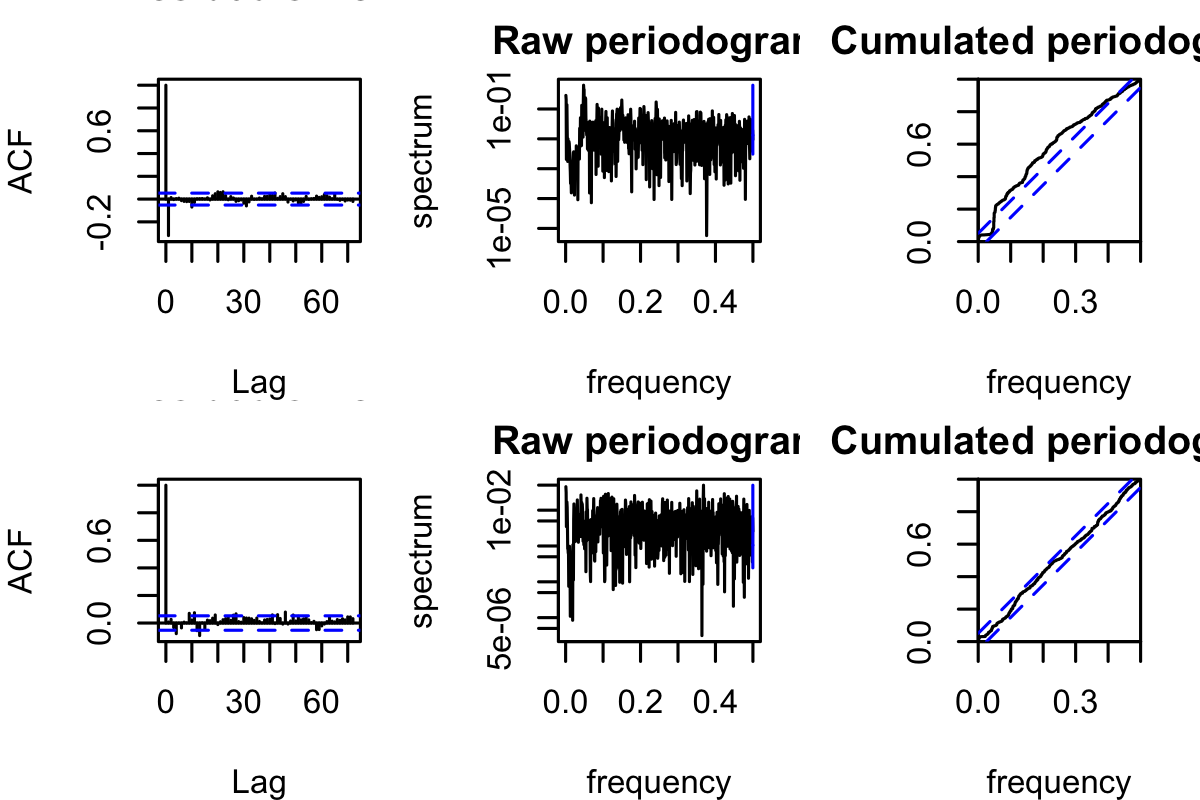
\includegraphics[width=\columnwidth]{figures/4thOrderModelValidation.png}
    \caption{...}
    \label{fig:4thOrderModelValidation}
\end{figure}


\subsubsection{Going from ON/OFF control to steady-state control}

Other benefits include more optimal use of the heat in the furnace by being able to integrate the dipping schedule to power consumption. Furthermore, smarter planning of the lid can be achieved by utilizing a more granular control of the power source. This kind of feed forward planning is possible due to continuos control.

\begin{figure}[!t]
    \centering
    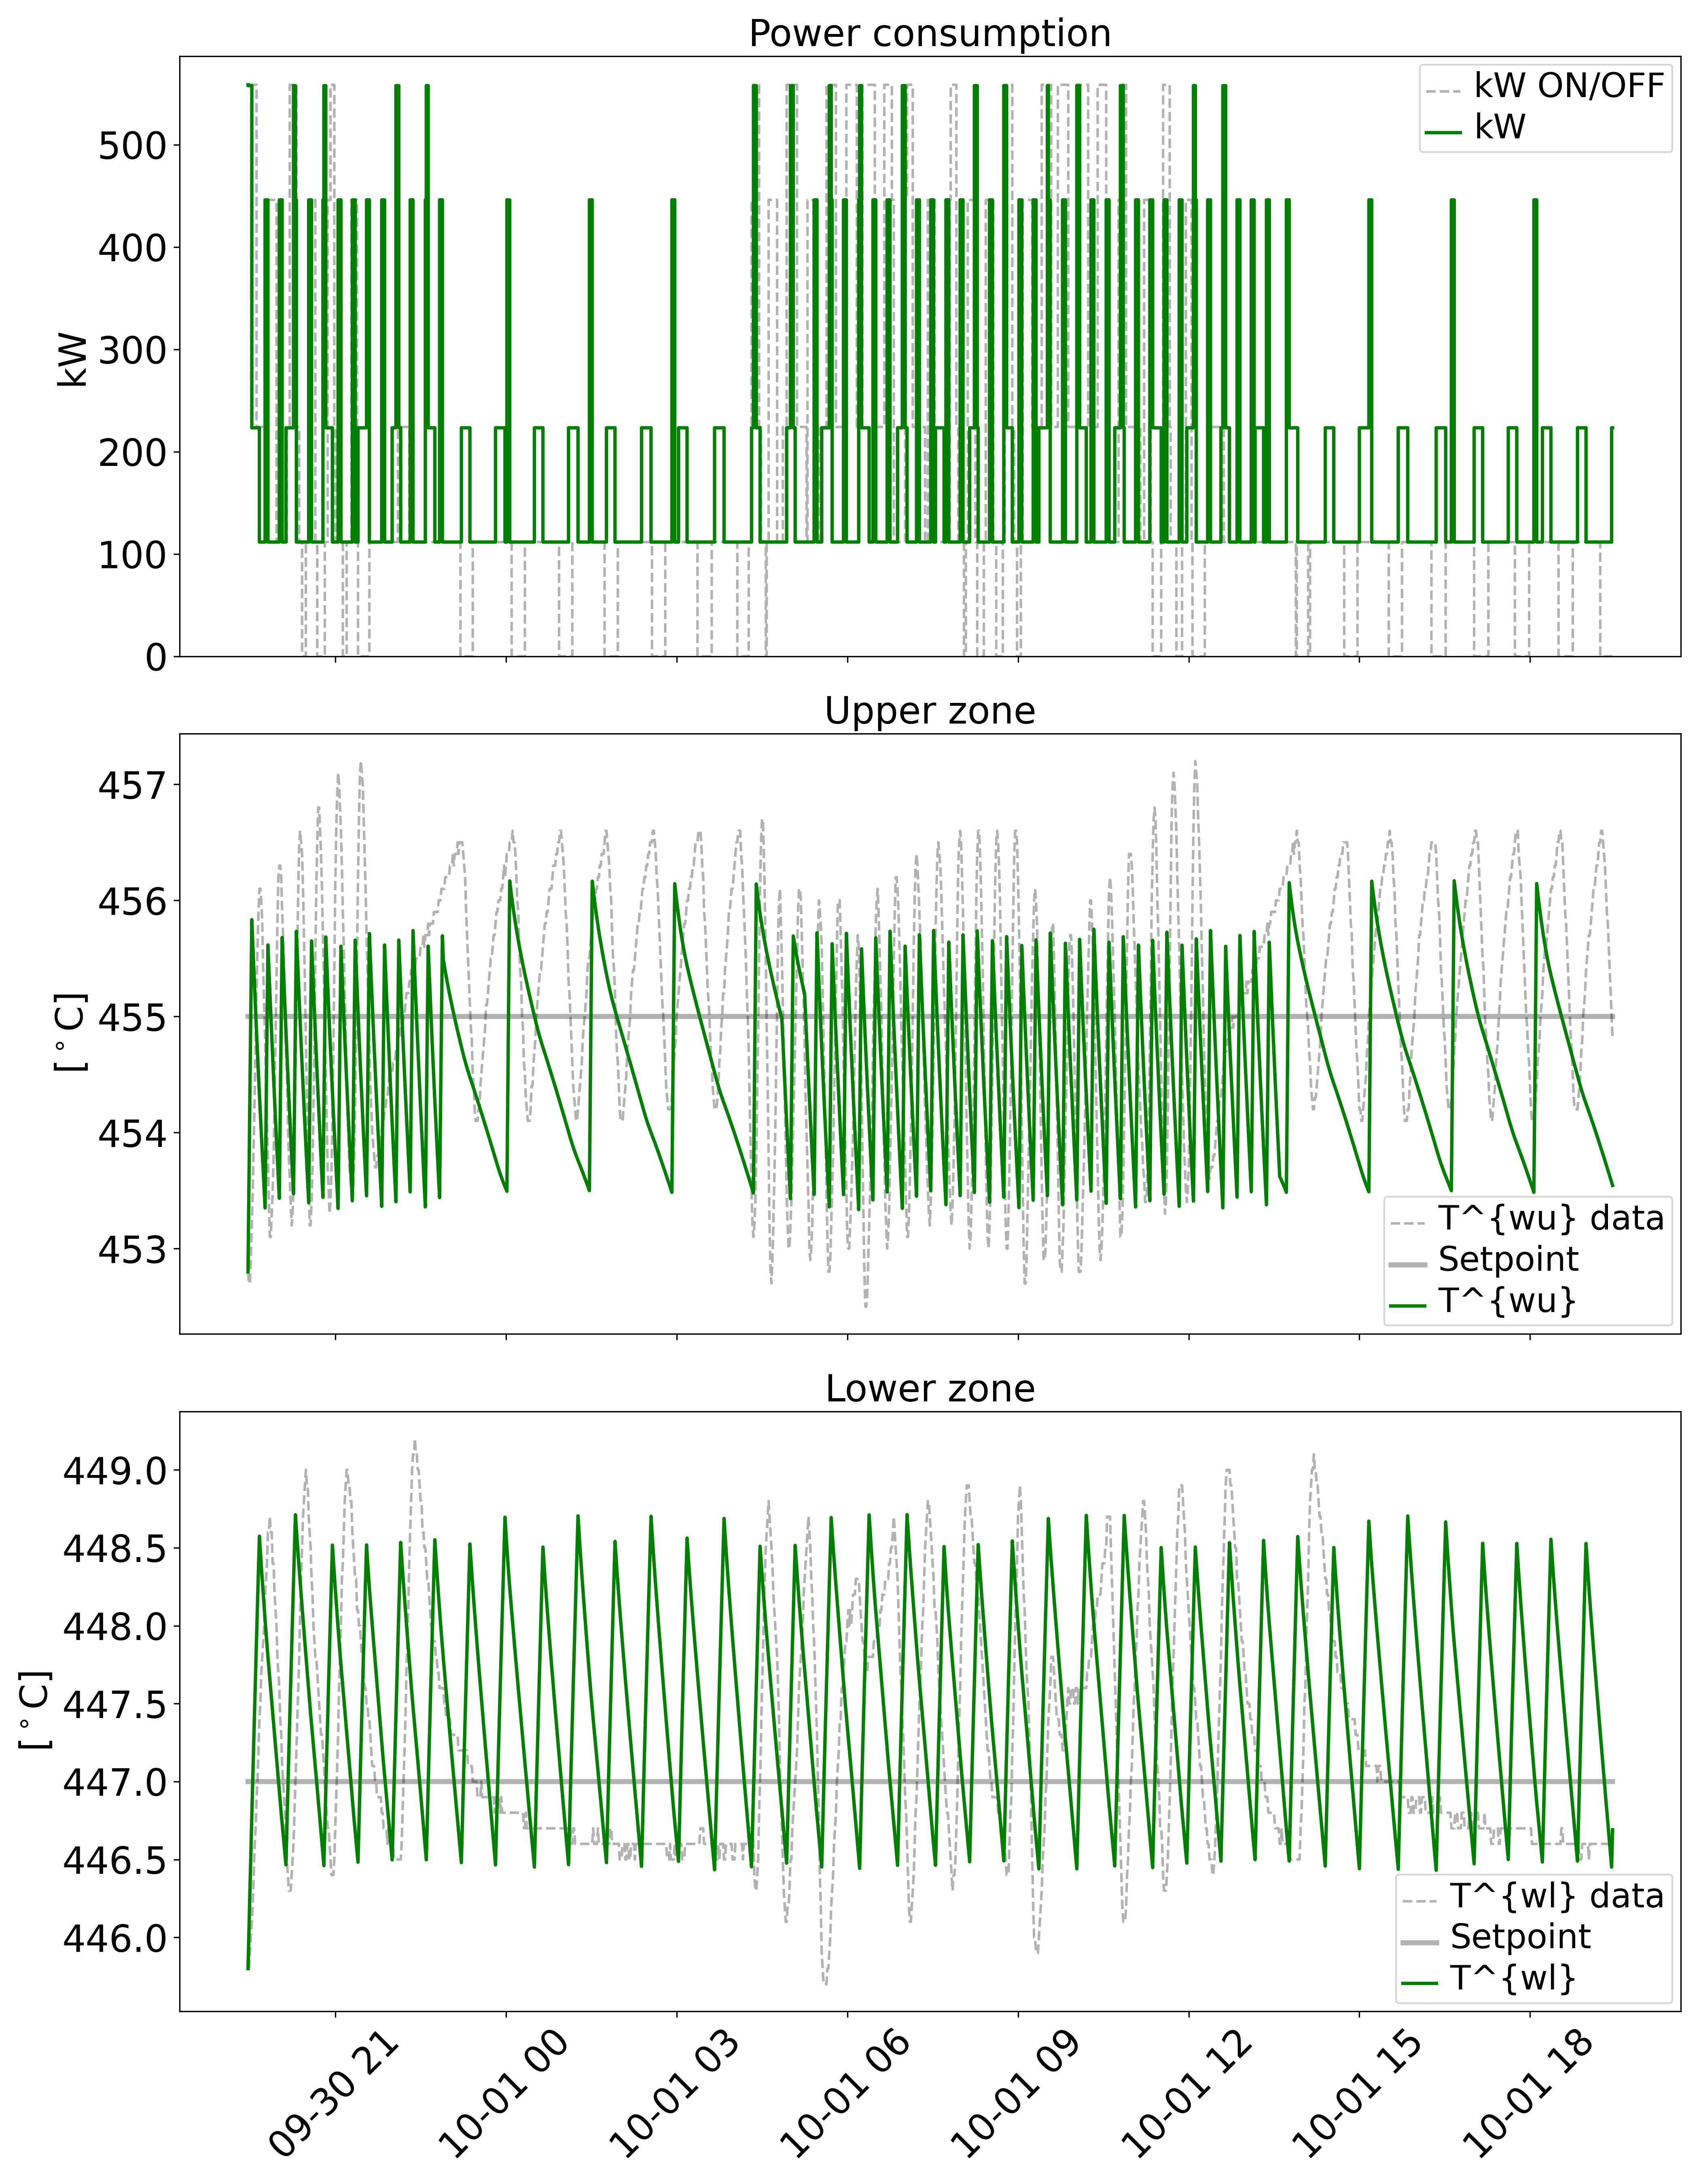
\includegraphics[width=\columnwidth]{figures/4thOrderModelVisualization.png}
    \caption{...}
    \label{fig:4thOrderModelVisualization}
\end{figure}

\section{Optimization model}


\section{Results}


\begin{figure}[!t]
    \centering
    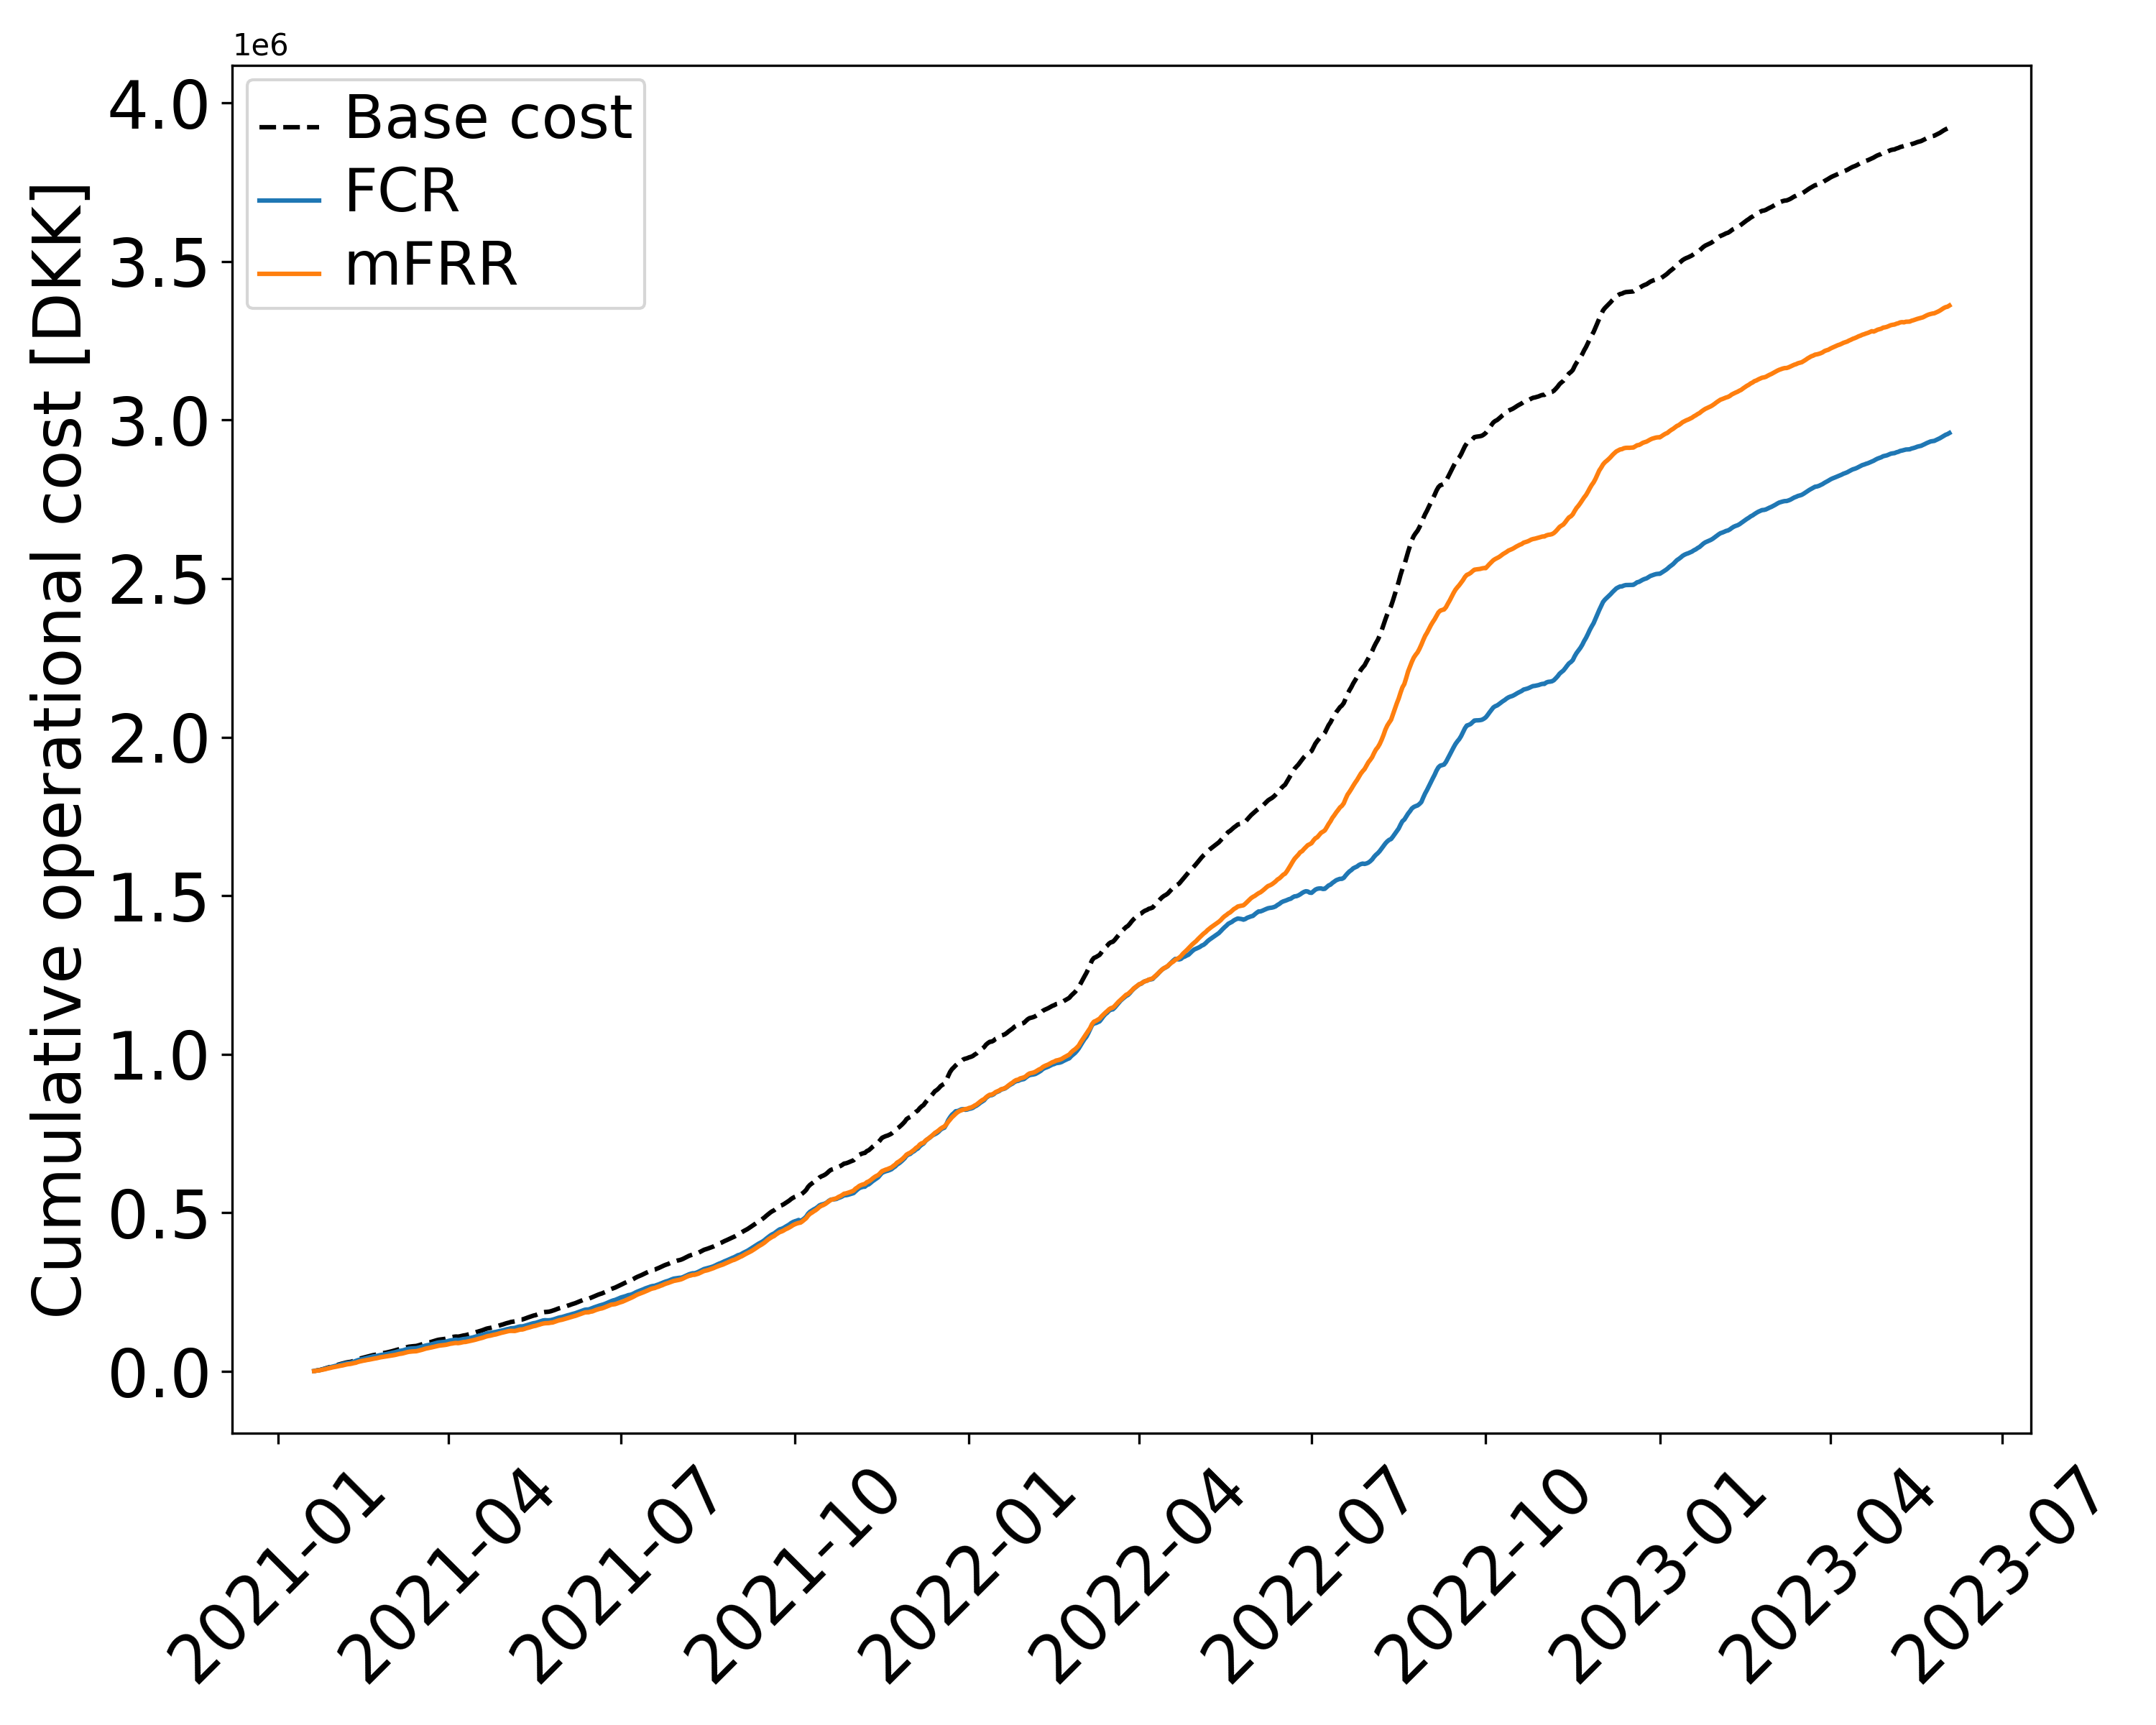
\includegraphics[width=\columnwidth]{figures/cumulative_cost_comparison.png}
    \caption{...}
    \label{fig:cumulative_cost_comparison}
\end{figure}

\begin{figure}[!t]
    \centering
    \includegraphics[width=\columnwidth]{figures/mfrr_single_case.png}
    \caption{...}
    \label{fig:mfrr_single_case}
\end{figure}

\begin{figure}[!t]
    \centering
    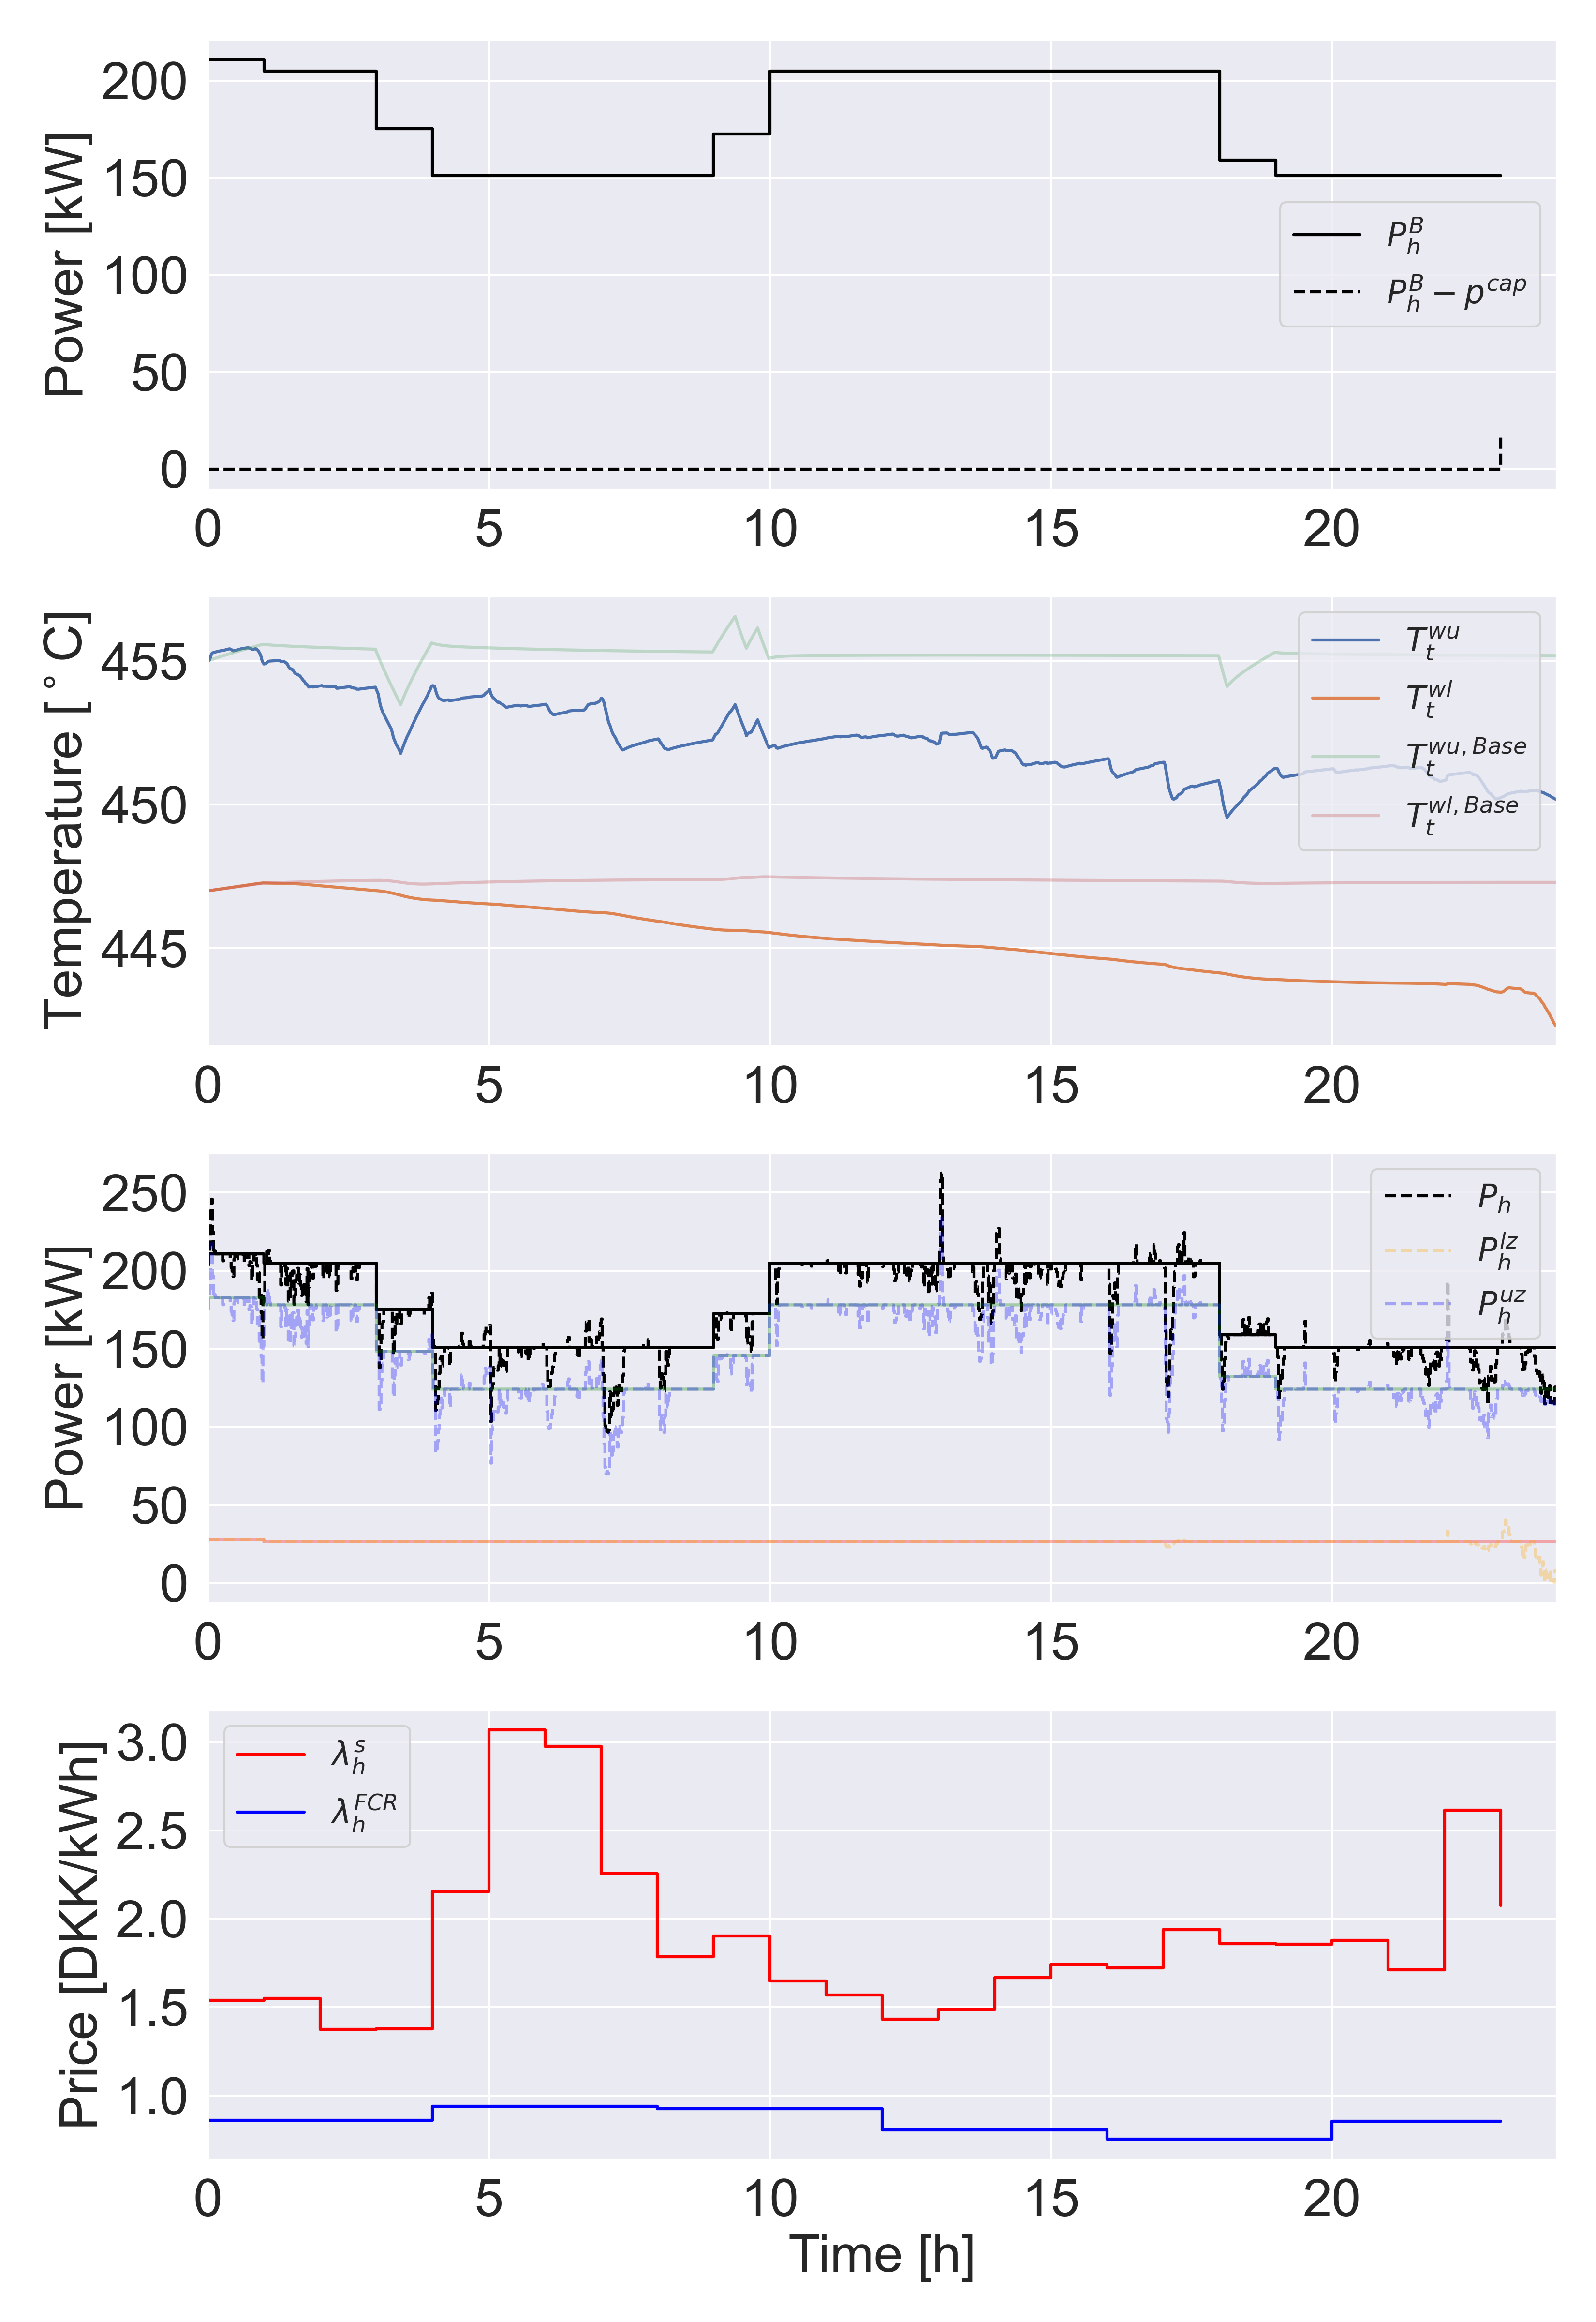
\includegraphics[width=\columnwidth]{figures/fcr_single_case.png}
    \caption{...}
    \label{fig:fcr_single_case}
\end{figure}

\section{Conclusion}



% \input{sections/appendix}

\section*{Acknowledgement}

The authors would like to acknowledge the financial support from Innovation Fund Denmark under grant number 0153-00205B for partially funding the work in this paper. The authors would also like to thank Haris Ziras (DTU) for his feedback on the paper and his valuable input on the development of the grey-box model of the freezer. The authors would also like to thank Coop and AK-Centralen for providing the freezer and power data from a supermarket used in this paper.

% The authors would also like to thank Christian Ahn Albertsen (IBM Client Innovation Center) for all our discussions and his feedback which has been particularly valuable regarding practical challenges faced for demand-response. The authors would also like to thank Bennevis Crowley (DTU) for reading the paper and providing feedback on corrections, figures, and phrases. The authors would also like to thank the Centre for Utilities and Supply at Energistyrelsen (Danish Energy Agency) for allowing us to present our work to them while also elaborating their perspective on Market Model 3.0 and their intentions.



\bibliographystyle{IEEEtran}
\bibliography{tex/bibliography/Bibliography.bib}

% \newpage

% \begin{IEEEbiographynophoto}{Peter A.V. Gade}
%     is an Industrial PhD researcher at IBM and affiliated with the Technical University of Denmark, Kongens Lyngby, Denmark, in the Energy Markets and Analytics Section within the Power and Energy Systems division at the Wind and Energy Systems Department. His research focuses on demand-side flexibility and the revenue streams from utilization of demand-side flexibility. He holds a M.S. in Mathematical Modelling and Computing and a B.S. in Biomedical Engineering, both from the Technical University of Denmark.
% \end{IEEEbiographynophoto}
% \begin{IEEEbiographynophoto}{Trygve Skjøtskfit}
%     is an Associate Partner at IBM Denmark, with focus on energy transformation and demand-side flexibility. His solid experience and deep knowledge within intelligent energy systems, buildings, and civil infrastructures makes him a leading figure, strategic advisor, and a first mover in the flexibility market with a strong track record to find and deliver new cutting-edge solutions. He holds an MBA in Strategy from Universitat Pompeu Fabra, and a Master of Export Engineering from Copenhagen University, College of Engineering.
% \end{IEEEbiographynophoto}
% \begin{IEEEbiographynophoto}{Henrik W. Bindner}
%     received the MSc in Electrical Engineering from Technical University of Denmark in 1988. He is currently a senior researcher with the Department of Wind and Energy Systems, Technical University of Denmark. He is heading the \textit{Distributed Energy Systems} Section and his research interests include control and management of smart grids, active distribution networks, and integrated energy systems.
% \end{IEEEbiographynophoto}
% \begin{IEEEbiographynophoto}{Charalampos Ziras}
%     ...
% \end{IEEEbiographynophoto}
% \begin{IEEEbiographynophoto}{Jalal Kazempour}
%     is an Associate Professor with the Department of Wind and Energy Systems, Technical University of Denmark, where he is heading the \textit{Energy Markets and Analytics} Section. He received the Ph.D. degree in Electrical Engineering from the University of Castilla-La Mancha, Ciudad Real, Spain, in 2013. His research interests include intersection of multiple fields, including power and energy systems, electricity markets, optimization, game theory, and machine learning.
% \end{IEEEbiographynophoto}


\vfill

\end{document}
